\chapter{Plotting}
\setlx\ provides a small plotting library which is based on \href{http://www.jfree.org/jfreechart/}{JFreeChart}.
The \setlx-interface to \textsl{JFreeChart} has been implemented by Arne R�cke and Fabian Wohriska.
The plotting library in \setlx\ supports three different kinds of plots:
\begin{enumerate}
\item The library can be used to plot curves.  Essentially, when it comes to curves, there are two kinds of curves:
      \begin{enumerate}
      \item Curves that are given as the
            \href{https://en.wikipedia.org/wiki/Graph_of_a_function}{\emph{graph of a function}}.  In
            this case, the $y$-coordinate is given as an expression involving the $x$-coordinate.  For example, the 
            \href{https://en.wikipedia.org/wiki/Parabola}{\emph{parabola}} satisfies the equation $y = x^2$. 
      \item Curves that are given via a 
            \href{https://en.wikipedia.org/wiki/Parametric_equation}{\emph{parametric equations}}.
            For example, a \href{https://en.wikipedia.org/wiki/Circle}{\emph{circle}} of radius 1
            can be specified via the parametric equations 
            \\[0.2cm]
            \hspace*{1.3cm}
            $x = \cos(t)$ \quad and \quad $y = \sin(t)$, \quad where $t \in [0, 2 \cdot \pi]$.
            \\[0.2cm]
            These equations specify a circle because $x^2 + y^2 = \cos^2(x) + \sin^2(x) = 1$.
      \end{enumerate}
      Both of these types of curves can be plotted by \setlx.
\item The library can be used for \href{https://en.wikipedia.org/wiki/Scatter_plot}{\emph{scatter plots}}.
\item The library can be used to plot \href{https://en.wikipedia.org/wiki/Chart}{\emph{statistical charts}} such as 
      \href{https://en.wikipedia.org/wiki/Bar_chart}{\emph{bar charts}} or 
      \href{https://en.wikipedia.org/wiki/Pie_chart}{\emph{pie charts}}.
\end{enumerate}
We will discuss the plotting of curves, scatter plots, and charts in different sections.

It should be noted that the figures presented in this tutorial had to be scaled down to fit the paper
size.  This scaling has resulted in a considerable loss of their artistic quality.

\section{Plotting Curves}
In this section, we discuss the plotting of mathematical curves.  The section is structured as
follows.
\begin{enumerate}
\item First, we discuss curves that are given as the graph of a function.
      As an example, we show how to plot the parabola.  
\item Next, we discuss curves that are specified via parametric equations.  As a simple example, we show how to
      plot a circle.  A second example discusses the plotting of a
      \href{https://en.wikipedia.org/wiki/Hypotrochoid}{\emph{hypotrochoid}}. 
\end{enumerate}
\subsection{Plotting the Parabola}
In order to start drawing, we first have to create a canvas on which we can draw  something.  This is achieved with
the command
\\[0.2cm]
\hspace*{1.3cm}
\texttt{c := plot\_createCanvas();}
\\[0.2cm]
Note that all functions related to plotting start with the prefix ``\texttt{plot\_}''.  The
function
\\[0.2cm]
\hspace*{1.3cm}
 ``\texttt{plot\_createCanvas}'' 
\\[0.2cm]
takes one optional argument, which is a string.  This string adds a title to the canvas.  For example, the command 
\\[0.2cm]
\hspace*{1.3cm}
\texttt{c := plot\_createCanvas(\symbol{34}The Parabola\symbol{34});} 
\\[0.2cm]
creates a canvas with the title ``\textsl{The Parabola}'' and returns a reference to this canvas.
However, as long as nothing is
painted on the canvas, the canvas remains invisible.  Let us draw a parabola on the canvas
created previously.  This is done using the command
\\[0.2cm]
\hspace*{1.3cm}
\texttt{plot\_addGraph(c, \qote{x*x}, \qote{f(x) = x*x}, [0, 0, 255]);}
\\[0.2cm]
The resulting figure is shown in Figure \ref{fig:parabola1.eps} on page \pageref{fig:parabola1.eps}.
The arguments provided to the function \texttt{plot\_addGraph} are interpreted as follows:
\begin{enumerate}
\item \texttt{c} refers to the canvas on which the specified function is to be drawn.
\item \texttt{\qote{x*x}} specifies the function.  The string given as argument
      is evaluated for different values of the variable $x$ and the resulting function is then
      plotted. 
\item \texttt{\qote{f(x) = x*x}} is the string that is used as the legend of the plot.  This string
      is printed verbatim below the plot.
\item \texttt{[0, 0, 255]} specifies the color used to plot the specified function.  This
      color is specified via the \href{https://en.wikipedia.org/wiki/RGB_color_model}{RGB color model}.
      Hence, in this case the parabola is plotted using the color blue.

      This parameter is optional.  If it is not specified, the curve will be plotted in black.
\item There is a final optional parameter to the function \texttt{plot\_addGraph} that is not
      used in this example.  This parameter needs to be a Boolean value.  If this value is
      \texttt{true}, then the area under the curve is filled with the specified color.
\end{enumerate}

\begin{figure}[!ht]
  \centering
  \epsfig{file=parabola1.eps, scale=0.6}
  \caption{A plot of the parabola $x \mapsto x^2$.}
  \label{fig:parabola1.eps}
\end{figure}

In Figure \ref{fig:parabola1.eps} the parabola is plotted for arguments ranging from $x = -10$ up to
$x = 10$.  Suppose that we would prefer to draw the parabola in the region where $x$ runs from $-4$
to $+4$.  We can use the function \texttt{plot\_modscale} to achieve this as follows:
\\[0.2cm]
\hspace*{1.3cm}
\texttt{plot\_modScale(c, [-4, 4], [-1,17]);}
\\[0.2cm]
The parameters used by \texttt{plot\_modScale} are as follows:
\begin{enumerate}
\item \texttt{c} specifies the canvas whose scale is to be modified.
\item \texttt{[-4, 4]} specifies that the $x$-coordinate is to be varied between $-4$ and $+4$.
\item \texttt{[-1, 17]} specifies that the $y$-coordinate extends from $-1$ to $+17$.
\end{enumerate}
The resulting parabola is shown in Figure \ref{fig:parabola2.eps} on page \pageref{fig:parabola2.eps}.

\begin{figure}[!ht]
  \centering
  \epsfig{file=parabola2.eps, scale=0.6}
  \caption{A plot of the parabola $x \mapsto x^2$.}
  \label{fig:parabola2.eps}
\end{figure}

Let us assume we want both the $x$-axis and the $y$-axis to be visible.  For this purpose, the
function \texttt{plot\_addListGraph} comes in handy.  To plot the $x$-axis we use the command
\\[0.2cm]
\hspace*{1.3cm}
\texttt{plot\_addListGraph(c, [[-4,0], [4,0]], \qote{x-axis}, [0,0,0]);}
\\[0.2cm]
Here, the parameters are as follows:
\begin{enumerate}
\item \texttt{c} specifies the canvas where we want to draw the line.
\item \texttt{[[-4,0], [4,0]]} is a list of points.  Each point is specified as a pair of $x$-
      and $y$-coordinates.  These points are then connected by straight lines.  In this case, as there is only one
      pair of points there is only one line.
\item \qote{x-axis} specifies the legend that is used for this line.
\item \texttt{[0,0,0]} specifies the color of the line.  This parameter is optional.
      If the color is not specified, then black is the default.
\end{enumerate}
Let us add the $y$-axis using the command
\\[0.2cm]
\hspace*{1.3cm}
\texttt{plot\_addListGraph(c, [[0,-1], [0,17]], \qote{y-axis});}
\\[0.2cm]
Furthermore, let us add a tangent to the parabola at the point $\pair(1,1)$.  Since the tangent line
at this point is given by the formula
\\[0.2cm]
\hspace*{1.3cm}
$x \mapsto 2 \cdot(x-1) + 1$,
\\[0.2cm]
the tangent line passes the points $\pair(-4, -9)$ and $\pair(4,7)$, Therefore, we can plot the tangent
using the command
\\[0.2cm]
\hspace*{1.3cm}
\texttt{plot\_addListGraph(c, [[-4,-9], [4,7]], \qote{x |-> 2*(x-1)+1});}
\\[0.2cm]
Finally, let us mark the point $\pair(1,1)$ with a tiny red box using the command
\\[0.2cm]
\hspace*{1.3cm}
\texttt{plot\_addBullets(c, [[1,1]], [255,0,0], 3.0);}
\\[0.2cm]
This command accepts four parameters.
\begin{enumerate}
\item \textrm{c} specifies the canvas.
\item \texttt{[[1,1]]} is a list of points.  Each point itself is specified as a pair of $x$- and $y$-
      coordinates. The function plots a square at the location of each of the points.
\item \texttt{[255,0,0]} specifies the color.
\item The last parameter specifies the size of each box.  This parameter is optional and
      defaults to $5.0$.  Note that this parameter has to be specified as a floating point number.
\end{enumerate}
The resulting graphics is shown in Figure \ref{fig:parabola3.eps} on page
\pageref{fig:parabola3.eps}.


\begin{figure}[!ht]
  \centering
  \epsfig{file=parabola3.eps, scale=0.6}
  \caption{A plot of the parabola $x \mapsto x^2$ and a tangent touching it.}
  \label{fig:parabola3.eps}
\end{figure}


The program used to create this plot showing the parabola is shown in Figure \ref{fig:parabola.stlx}
on page \pageref{fig:parabola.stlx}.  This program contains three lines the we have not yet
discussed.
\begin{enumerate}
\item Line 2 contains a call to the function \texttt{sleep}.  This call is necessary if we want to
      run this program from the command line.  The reason is that the function
      \texttt{plot\_createCanvas} runs concurrently to the rest of the program.  However, the invocation
      of the function \texttt{plot\_addGraph} in line 3 uses the canvas created in line 1.  If the
      creation of this canvas has not been finished, the \textsl{Java} runtime system that is lying
      beneath \setlx\ might create a \emph{concurrent modification exception}.  By calling
      \texttt{sleep} the execution of the main thread of the program is halted for 100 milliseconds.
      This should be more than enough for the function \texttt{plot\_createCanvas} to finish its
      work. 
\item Line 9 exports the plot into a
      \href{https://en.wikipedia.org/wiki/Portable_Network_Graphics}{\texttt{png}-file} named
      \texttt{parabola.png}.  This file is saved into the current directory.
\item Finally, we have to prevent the \setlx\ interpreter from exiting after it has finished
      displaying the parabola.  This is achieved via the invocation of \texttt{get} in line 10.
      The command \texttt{get} waits for the user to enter any string.  Therefore, as long as the
      user does not press \texttt{$\langle$Enter$\rangle$}, the window showing the parabola remains visible. 
\end{enumerate}

\begin{figure}[!ht]
\centering
\begin{Verbatim}[ frame         = lines, 
                  framesep      = 0.3cm, 
                  firstnumber   = 1,
                  labelposition = bottomline,
                  numbers       = left,
                  numbersep     = -0.2cm,
                  xleftmargin   = 0.8cm,
                  xrightmargin  = 0.8cm,
                ]
    c := plot_createCanvas("The Parabola");
    sleep(100);
    plot_addGraph(c, "x*x", "f(x) = x*x", [0, 0, 255]);
    plot_modScale(c, [-4, 4], [-1,17]);
    plot_addListGraph(c, [[-4, 0], [4, 0]], "x-axis", [0,0,0]);
    plot_addListGraph(c, [[ 0,-1], [0,17]], "y-axis");
    plot_addListGraph(c, [[-4,-9], [4, 7]], "x |-> 2*(x-1)+1", [0,255,0]);
    plot_addBullets(c, [[1,1]], [255,0,0], 3.0);
    plot_exportCanvas(c, "parabola");
    get("Press Enter to continue");
\end{Verbatim}
\vspace*{-0.3cm}
\caption{\setlx\ commands to plot the parabola.}
\label{fig:parabola.stlx}
\end{figure}

\subsection{Plotting Parametric Curves}
Next, we show how to plot a parametric curve.  
As a first example, we show how to plot a circle of radius 1.  Figure \ref{fig:circle.stlx} on page
\pageref{fig:circle.stlx} shows a \setlx\ program that can be used to plot a circle.  The resulting
circle is shown in Figure \ref{fig:circle.eps} on page \pageref{fig:circle.eps}.

\begin{figure}[!ht]
\centering
\begin{Verbatim}[ frame         = lines, 
                  framesep      = 0.3cm, 
                  firstnumber   = 1,
                  labelposition = bottomline,
                  numbers       = left,
                  numbersep     = -0.2cm,
                  xleftmargin   = 0.8cm,
                  xrightmargin  = 0.8cm,
                ]
    c := plot_createCanvas("The Unit Circle");
    sleep(100);
    interval := [0, 2*mathConst("Pi")];
    blue     := [0, 0, 255];
    plot_addParamGraph(c, "cos(x)", "sin(x)", "circle", interval, blue);
    plot_addListGraph(c, [[-2, 0], [2, 0]], "x-axis", [0,0,0]);
    plot_addListGraph(c, [[ 0,-2], [0, 2]], "y-axis");
    plot_modScale(c, [-1.2, 1.2], [-1.2, 1.2]);
    plot_modSize(c, [600, 600]);
    plot_exportCanvas(c, "circle");
    get("Press Enter to continue");
\end{Verbatim}
\vspace*{-0.3cm}
\caption{The unit circle.}
\label{fig:circle.stlx}
\end{figure}


\begin{figure}[!ht]
  \centering
  \epsfig{file=circle.eps, scale=0.6}
  \caption{A plot of the unit circle satisfying  $x^2 + y^2 = 1$.}
  \label{fig:circle.eps}
\end{figure}

We proceed to discuss the program shown in Figure \ref{fig:circle.stlx} line by line.
\begin{enumerate}
\item Line 1 creates the canvas and equips it with a title.
\item Line 2 waits for the canvas to be created.
\item According to the \href{https://en.wikipedia.org/wiki/Pythagorean_theorem}{Pythagorean theorem}
      the points $\pair(x,y)$ on a unit circle satisfy the equation
      \\[0.2cm]
      \hspace*{1.3cm}
      $x^2 + y^2 = 1^2$.
      \\[0.2cm]  
      Since we have $\sin^2(\varphi) + \cos^2(\varphi) = 1$, the set of all points on the unit
      circle is given as
      \\[0.2cm]
      \hspace*{1.3cm}
      $\bigl\{\langle \cos(\varphi), \sin(\varphi) \rangle : \varphi \in [0, 2 \cdot \pi] \bigr\}$.
      \\[0.2cm]
      Therefore, we specify the variable \texttt{interval} as the pair \texttt{[0, 2*mathConst(\qote{Pi})]} 
      since this variable is used to specify the range over which the parameter has to vary.
\item Line 4 specifies the color.
\item Line 5 calls the function \texttt{addParamGraph} to do the actual plotting.  The parameters to
      this function are as follows:
      \begin{enumerate}
      \item \texttt{c} is the canvas on which the curve is to be plotted.
      \item \texttt{\qote{cos(x)}} specifies the function computing the $x$-coordinate. 
      \item \texttt{\qote{sin(x)}} specifies the function computing the $y$-coordinate. 
      \item \texttt{\qote{circle}} specifies the legend.
      \item \texttt{interval} specifies the range over which the variable \texttt{x} that is used in 
            the expressions \texttt{\qote{cos(x)}} and \texttt{\qote{sin(x)}} has to vary.
      \item \texttt{blue} specifies the color.  This argument is optional.
      \end{enumerate}
\item Line 6 plots the $x$-axis.
\item Line 7 plots the $y$-axis.
\item Line 8 specifies that the region to be plotted ranges from $x=-1.2$ to $x=1.2$ horizontally
      and form $y=-1.2$ to $y=1.2$ vertically. 
\item Line 9 changes the size of the plot.  By default, a canvas is $800$ pixels wide and $600$
      pixels high.  Plotting a circle on a canvas with these dimensions would distort the circle and
      make it look like an \href{https://en.wikipedia.org/wiki/Ellipse}{\emph{ellipse}}.  In order to plot a proper circle we therefore have to ensure
      that the canvas is quadratic.  Hence we change the plotting area to be $600$ pixels wide and
      $600$ pixels high. 
\item Line 10 saves the generated plot into a file.
\item Line 11 prevents the program from finishing prematurely.
\end{enumerate}


\begin{figure}[!ht]
\centering
\begin{Verbatim}[ frame         = lines, 
                  framesep      = 0.3cm, 
                  firstnumber   = 1,
                  labelposition = bottomline,
                  numbers       = left,
                  numbersep     = -0.2cm,
                  xleftmargin   = 0.0cm,
                  xrightmargin  = 0.0cm,
                ]
    period := procedure(bigR, smallR) {
        for (i in [1 ..10000]) {
            if (isInteger(i * (bigR - smallR) / (smallR* 2))) {
                return i;
            }
        }
        return 1000;
    };
    hypotrochoid := procedure(bigR, smallR, d) {
        c := plot_createCanvas("The Hypotrochroid R=$bigR$, r=$smallR$, d=$d$.");
        sleep(100);
        interval := [0, 2.01*mathConst("Pi")*period(bigR, smallR)];
        red      := [255, 0, 0];
        sum      := (bigR - smallR + d) + 0.5;
        xParam   := "(bigR-smallR) * cos(x) + d * cos(x*(bigR-smallR)/smallR)";
        yParam   := "(bigR-smallR) * sin(x) - d * sin(x*(bigR-smallR)/smallR)";
        plot_addParamGraph(c, xParam, yParam, "hypotrochoid", interval, red);
        plot_addListGraph(c, [[-sum,   0], [sum,   0]], "x-axis", [0,0,0]);
        plot_addListGraph(c, [[   0,-sum], [  0, sum]], "y-axis");   
        plot_modScale(c, [-sum, sum], [-sum, sum]);
        plot_modSize(c, [600, 600]);
        plot_exportCanvas(c, "hypotrochoid");
        get("Press Enter to continue");
    };
\end{Verbatim}
\vspace*{-0.3cm}
\caption{A program for plotting Hypotrochoids.}
\label{fig:hypotrochoid.stlx}
\end{figure}

As another example let us write a program for plotting 
\href{https://en.wikipedia.org/wiki/Hypotrochoid}{\emph{hypotrochoids}}.  These curves are described
by the equations
\\[0.2cm]
\hspace*{1.3cm}
$\displaystyle x = (R - r) \cdot \cos(\varphi) + d \cdot \cos\Bigl(\varphi \cdot
\frac{R-r}{r}\Bigr)$ \quad and \quad
$\displaystyle y = (R - r) \cdot \sin(\varphi) - d \cdot \sin\Bigl(\varphi \cdot\frac{R-r}{r}\Bigr)$.
\\[0.2cm]
Here, $\varphi$ has to run form $0$ up to some number $\Phi$ such that $\Phi$ is a multiple of $2\cdot\pi$
and, furthermore, 
\\[0.2cm]
\hspace*{1.3cm}
$\displaystyle \Phi \cdot\frac{R-r}{r}$
\\[0.2cm]
has to be a multiple of $2 \cdot \pi$, too.  Figure \ref{fig:hypotrochoid.stlx} on page \pageref{fig:hypotrochoid.stlx}
shows a \setlx\ program that can be used to plot a hypotrochoid.  Figure \ref{fig:hypotrochoid.eps}
on page \pageref{fig:hypotrochoid.eps} shows the hypotrochoid where $R=5$, $r=3$ and $d=5$.
\begin{figure}[!ht]
  \centering
  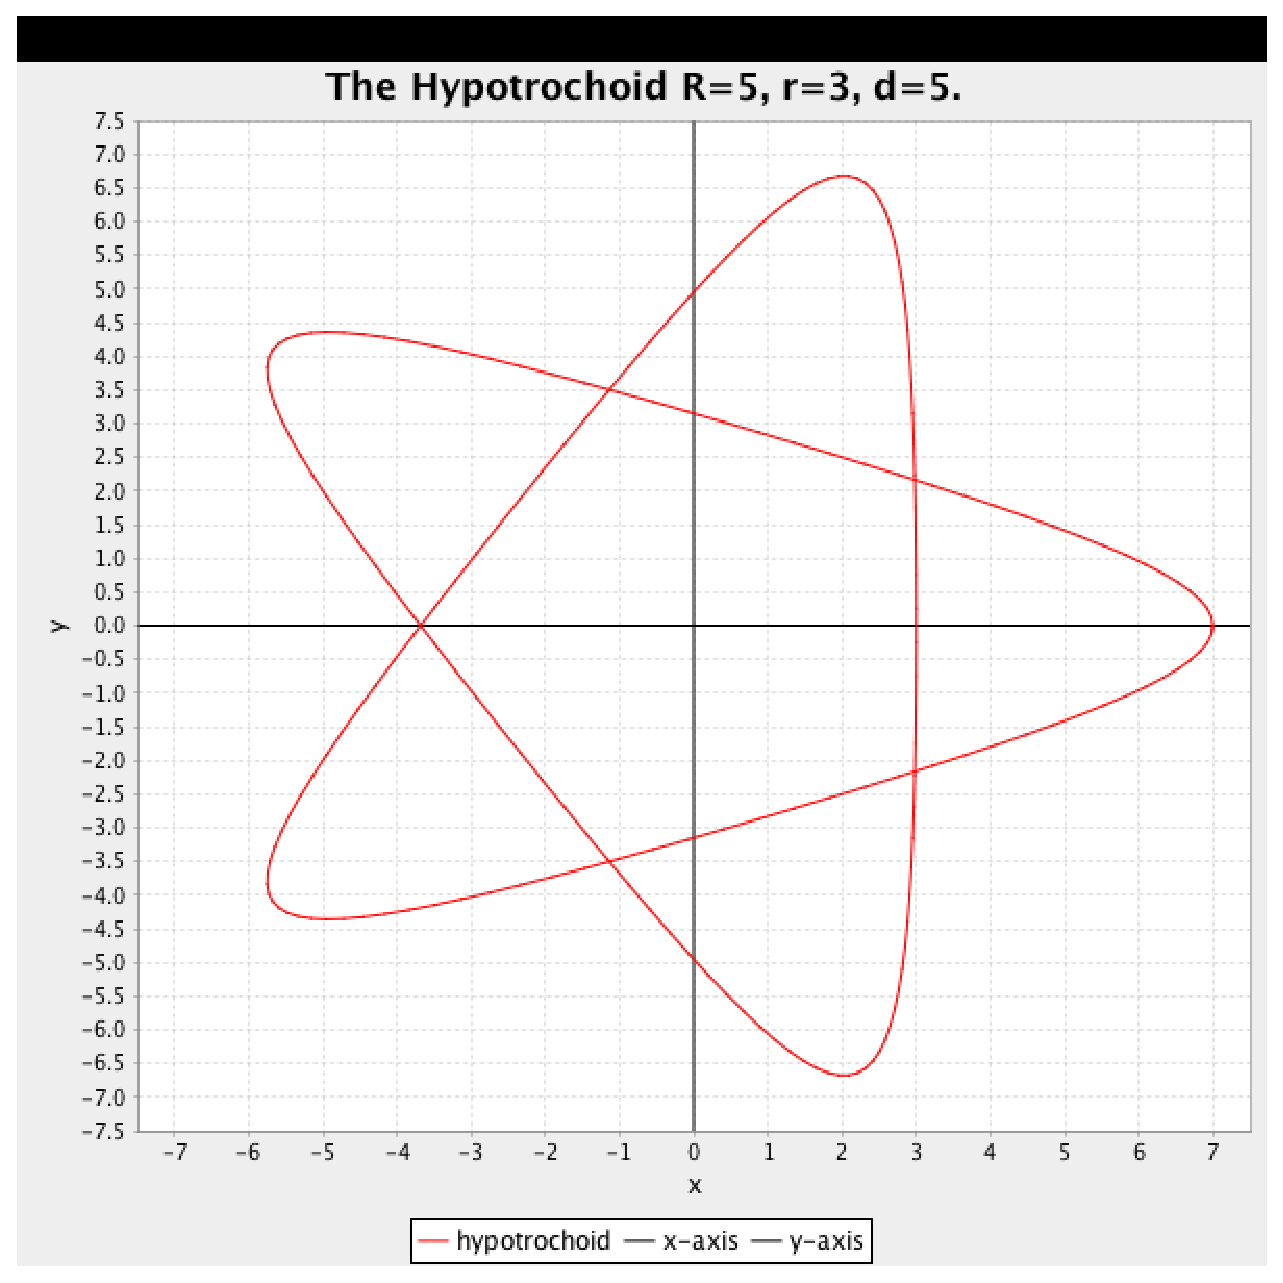
\epsfig{file=hypotrochoid.eps, scale=0.6}
  \caption{A plot of the hypotrochoid satisfying  $R = 5$, $r=3$, $d = 5$.}
  \label{fig:hypotrochoid.eps}
\end{figure}


\vspace*{\fill}
\pagebreak

\vspace*{\fill}
\pagebreak

\section{Scatter Plots}
In order to generate a \href{https://en.wikipedia.org/wiki/Scatter_plot}{scatter plot}, we can use
the function \texttt{plot\_addBullets}.  Figure \ref{fig:fathers-and-sons.stlx} on page
\pageref{fig:fathers-and-sons.stlx} shows the implementation of the function \texttt{fatherAndSons}
that reads a file containing the heights of fathers and their sons and that converts these data into
the scatter plot shown in Figure \ref{fig:fathers-and-sons.eps} on page
\pageref{fig:fathers-and-sons.eps}.  We proceed to discuss the details of the implementation of the
function \texttt{fatherAndSons}.
\begin{enumerate}
\item Line 2 reads the file ``\texttt{fathers-and-sons.txt}'' and converts this file into a list of
      strings that is called \texttt{data}.  Each string corresponds to one line in the file.
      The first line in the file has the form 
      \\[0.2cm]
      \hspace*{1.3cm}
      \texttt{65.04851 59.77827}
      \\[0.2cm]
      This line states that the first father-son pair in the data set consists of a father who is
      $65.04851$ inches tall, while his son is only $59.77827$ inches tall.\footnote{
        At this point you are probably wondering how it is possible that the height is measured with a
        precision of 5 digits.  Of course, when measuring body heights this is precision is not
        achievable.  The data set I am using here is part of
        the \href{http://www.r-project.org}{\texttt{R} project} and can be found in the package
        \\[0.2cm]
        \hspace*{1.3cm}
        \href{http://www.inside-r.org/packages/cran/UsingR/docs/father.son}{\texttt{UsingR}}
        \\[0.2cm]
        in the variable \texttt{father.son}. 
        My best guess is that the data set has suffered from some kind of unit conversion. 
      }.
\item Line 3 splits every string in the list \texttt{data} into a list of two strings.  These two
      strings are the strings representing the height of the father and the height of his son.
      Therefore, the variable \texttt{fsStr} is a list of pairs of strings.  These pairs correspond
      to the lines in the file ``\texttt{fathers-and-sons.txt}''.
\item Line 4 converts these strings into floating point values.  This is done using the conversion
      function \texttt{double} that takes a string and converts it into a floating point number.
\item Line 5 creates the canvas.
\item Line 6 takes the pairs  of floating point numbers and plots them as boxes of size $2.0$.
      Note that the size has to be specified as a floating point number:  Specifying the height as
      an integer will result in an error message.

      The function \texttt{plot\_addBullets} takes a list of pairs of the form $[x,y]$ where $x$
      specifies the $x$-coordinate and $y$ specifies the $y$-coordinate of a data point.  These data
      points are then plotted one by one.
\item As the heights vary between 58 inches and 80 inches, line 7 modifies the scale accordingly.
\item Line 8 modifies the size of the canvas so that the width and the height are the same.
\item Line 9 changes the labeling of the $x$-axis and of the $y$-axis using the function
      \texttt{plot\_labelAxis}.  This function takes three arguments.
      \begin{enumerate}
      \item The first  argument is the canvas.
      \item The second argument is the label of the $x$-axis.
      \item The third  argument is the label of the $y$-axis.
      \end{enumerate}
\item Line 10 saves the scatter plot into a file. The file is saved as a \texttt{.png} file.
\end{enumerate}



\begin{figure}[!ht]
\centering
\begin{Verbatim}[ frame         = lines, 
                  framesep      = 0.3cm, 
                  firstnumber   = 1,
                  labelposition = bottomline,
                  numbers       = left,
                  numbersep     = -0.2cm,
                  xleftmargin   = 0.0cm,
                  xrightmargin  = 0.0cm,
                ]
    fatherAndSons := procedure() {
        data  := readFile("fathers-and-sons.txt");
        fsStr := [ split(line, " "): line in data ];
        fs    := [ [double(x), double(y)] : [x,y] in fsStr ];
        c     := plot_createCanvas("Heights of Fathers vs. Heights of Sons.");
        plot_addBullets(c, fs, [0,0,255], 2.0);
        plot_modScale(c, [58, 80], [58, 80]);
        plot_modSize(c, [1000, 1000]);
        plot_labelAxis(c, "heights of fathers in inches", 
                          "heights of sons in inches"    );
        plot_exportCanvas(c, "fathers-and-sons");
    };
\end{Verbatim}
\vspace*{-0.3cm}
\caption{How to generate a scatter plot from data stored in a file.}
\label{fig:fathers-and-sons.stlx}
\end{figure}

\begin{figure}[!ht]
  \centering
  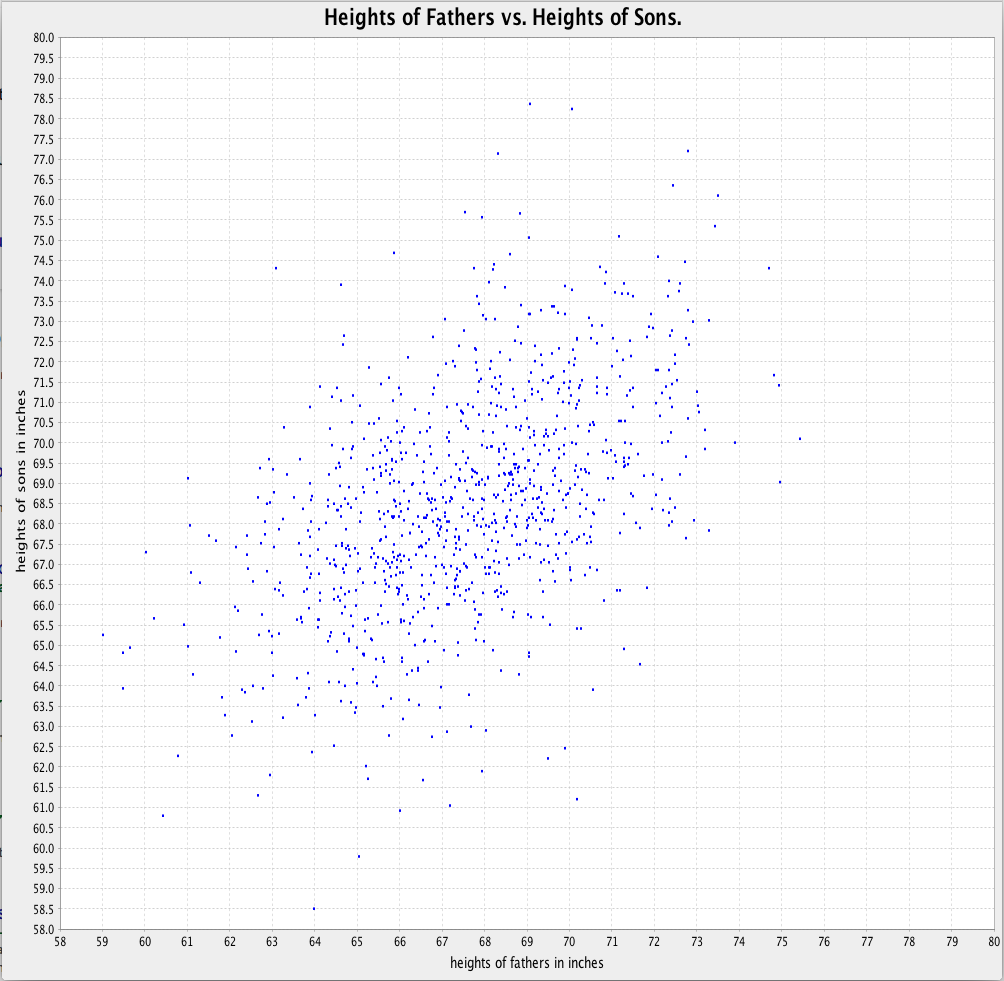
\epsfig{file=fathers-and-sons.eps, scale=0.4}
  \caption{A scatter plot showing the heights of fathers and their sons.}
  \label{fig:fathers-and-sons.eps}
\end{figure}

\vspace*{\fill}
\pagebreak


\section{Plotting Statistical Charts}
\setlx\ is able to draw \href{https://en.wikipedia.org/wiki/Bar_chart}{\emph{bar charts}} and
\href{https://en.wikipedia.org/wiki/Pie_chart}{\emph{pie charts}}.
We will present each of these charts in a separate subsection.

\subsection{Bar Charts}
\begin{table}
  \centering
  \begin{tabular}{|l|r|r|r|r|r|}
    \hline                                                     
    \diagbox{Region}{Year} & 1900 & 1950 & 1999 & 2008 & 2010 \\
    \hline                                                     
    \hline                                                     
    Northern America       &    82 &   172 &   307 &   337 &   345 \\
    \hline                                                      
    Oceania                &     6 &    13 &    30 &    34 &    37 \\
    \hline                                                     
    Latin America          &    74 &   167 &   511 &   577 &   590 \\
    \hline                                                     
    Europe                 &   408 &   547 &   729 &   732 &   738 \\ 
    \hline                                                     
    Africa                 &   133 &   221 &   767 &   973 & 1,022 \\ 
    \hline                                                     
    Asia                   &   947 & 1,402 & 3,634 & 4,054 & 4,164 \\
    \hline                                                     
    World                  & 1,650 & 2,521 & 5,978 & 6,707 & 6,896 \\
    \hline                                         
  \end{tabular}
  \caption{The world population in millions of people.}
  \label{tab:world-population}
\end{table}

\noindent
Table \ref{tab:world-population} on page \pageref{tab:world-population} shows the population of
different regions of the world for various years.  This data is more easily comprehensible when
presented as a bar char.  Figure \ref{fig:world-population.stlx} presents a \setlx-program that
converts these data into a bar chart.  We proceed to discuss this program line by line.
The bar chart produced by this program is shown in Figure \ref{fig:world-population.eps} on page
\pageref{fig:world-population.eps}.



\begin{figure}[!ht]
\centering
\begin{Verbatim}[ frame         = lines, 
                  framesep      = 0.3cm, 
                  firstnumber   = 1,
                  labelposition = bottomline,
                  numbers       = left,
                  numbersep     = -0.2cm,
                  xleftmargin   = 0.0cm,
                  xrightmargin  = 0.0cm,
                ]
    data := [ ["Year"            , 1900, 1950, 1999, 2008, 2010],
              ["Northern America",   82,  172,  307,  337,  345],
              ["Oceania"         ,    6,   13,   30,   34,   37],
              ["Latin America"   ,   74,  167,  511,  577,  590],
              ["Europe"          ,  408,  547,  729,  732,  738], 
              ["Africa"          ,  133,  221,  767,  973, 1022], 
              ["Asia"            ,  947, 1402, 3634, 4054, 4164],
              ["World"           , 1650, 2521, 5978, 6707, 6896] ];
    worldPopulation := procedure(data) {
        c       := plot_createCanvas();
        years   := data[1][2..];
        regions := [line[1]: line in data[2..]];
        for (i in [1..#years]) {
            population := [region[i+1] : region in data[2..]];
            plot_addBarChart(c, population, regions, "Population in $years[i]$");
        }
    };
    worldPopulation(data);
\end{Verbatim}
\vspace*{-0.3cm}
\caption{Program to plot the world population as a bar chart.}
\label{fig:world-population.stlx}
\end{figure}

\begin{enumerate}
\item Line 1 to line 8 define the data that is to be displayed.  The data is stored as a list of
      lists.  The first list specifies the years corresponding to the population counts.
      The remaining lists each specify the population counts for a specific geographical region.
\item The function \texttt{worldPopulation} has one parameter.  This parameter is of the form of the
      data specified in line 1 to line 8.
\item Line 10 creates the canvas.
\item Line 11 extracts the years.
\item Line 12 extract the regions from the first column of \texttt{data}.
\item Since our intention is to present the data of the different regions combined by the years, 
      we select these data in the list \texttt{population} in line 14.  Here, \texttt{region} iterates
      over the different regions in \texttt{data}, while \texttt{region[i+1]} selects the data for the $i$th
      year in the table.
\item The function \texttt{plot\_addBarChart} plots the bar chart. The arguments to this function 
      are as follows:
      \begin{enumerate}
      \item \texttt{c} specifies  the canvas.
      \item \texttt{population} is a list of numbers.  For every number in this list, the function 
            \texttt{plot\_addBarChart} plots a line of the corresponding height into each of the
            groups.  The groups are labeled by the list \texttt{regions}.  The lines plotted by one
            invocation of \texttt{plot\_addBarChart} all have the same unique color.  This color is
            determined automatically.
      \item \texttt{regions} is a list of strings specifying a label for each group.
      \item The last argument specifies a legend for the data plotted by this instance of 
            \texttt{plot\_addBarChart}.
      \end{enumerate}
\end{enumerate}
In order to understand what is plotted where, it is easiest to compare the variable \texttt{data} defined in Figure
\ref{fig:world-population.stlx} to the plot in Figure \ref{fig:world-population.eps}


\begin{figure}[!ht]
  \centering
  \epsfig{file=world-population.eps, scale=0.5}
  \caption{A Bar chart showing the world population in millions in different regions.}
  \label{fig:world-population.eps}
\end{figure}

\subsection{Pie Charts}
Table \ref{tab:race-prison} on Page \pageref{tab:race-prison} shows the distribution of
different races in the Texan population and in  the population of Texan prisons.  In order to
further our understanding of the data, let us visualize it via two pie charts.  The visualization is
achieved using the \setlx-program shown in Figure \ref{fig:race-and-incarceration.stlx} on page
\pageref{fig:race-and-incarceration.stlx}.  The resulting pie charts are shown in Figure 
\ref{fig:race-prison} on page \pageref{fig:race-prison}.  We proceed to discuss the \setlx-program.


\begin{table}[!hb]
  \centering
  \begin{tabular}{|l|r|r|}
    \hline
    Race  & Population & Prison Population \\
    \hline
    \hline
     white & 10933313 & 38396 \\
    \hline
    black  &  2404566 & 51649 \\
    \hline
    latino &  6669666 & 35028 \\
    \hline
    other  &   844275 &   582 \\
    \hline
  \end{tabular}
  \caption{The race distribution in the Texan population vs.~the Texan prison population.}
  \label{tab:race-prison}
\end{table}

\begin{figure}[!ht]
\centering
\begin{Verbatim}[ frame         = lines, 
                  framesep      = 0.3cm, 
                  firstnumber   = 1,
                  labelposition = bottomline,
                  numbers       = left,
                  numbersep     = -0.2cm,
                  xleftmargin   = 0.8cm,
                  xrightmargin  = 0.8cm,
                ]
    data := [ ["white", 10933313, 38396],
              ["black",  2404566, 51649],
              ["latino", 6669666, 35028],
              ["other",   844275,   582]
        ];
    prisonPopulation := procedure(data) {
        c1 := plot_createCanvas("Race disdribution in Texas.");
        c2 := plot_createCanvas("Race disdribution in Texan prisons.");
        races      := [line[1]: line in data];
        population := [line[2]: line in data];
        inmates    := [line[3]: line in data];
        plot_addPieChart(c1, population, races);
        plot_addPieChart(c2, inmates,    races);
        plot_exportCanvas(c1, "race-population");
        plot_exportCanvas(c2, "race-incarceration");
    };
\end{Verbatim}
\vspace*{-0.3cm}
\caption{A program to generate two pie charts.}
\label{fig:race-and-incarceration.stlx}
\end{figure}

\begin{enumerate}
\item The data are defined in line 1 to 5 as a list of list.  Each list in \texttt{data} corresponds
      to a different race. 
\item The procedure \texttt{prisonPopulation} takes this data as its sole input.
\item Line 7 and 8 create two different canvases for the two pie charts.
\item Line 9 extracts the different races stored in the table \texttt{data}.
\item Line 10 is defined as list containing the number of people of the various races living in
      Texas.
\item Line 11 is the corresponding list containing the number of prison inmates of each race.
\item Line 12 draws the pie chart showing the Texan race distribution via a call of the function
      \texttt{plot\_addPieChart}.
      \begin{enumerate}
      \item The first parameter specifies the canvas on which the pie chart is to be drawn.
      \item The second parameter is a list of numbers.
      \item The final parameter is a list of labels.
      \end{enumerate}
\item Line 13 draws the pie chart showing the  race distribution of Texan inmates.
\item The last two lines save the generated charts as \texttt{png} files.
\end{enumerate}

\begin{figure}[!ht]
  \centering
  \epsfig{file=race-population.eps, scale=0.6}
  \epsfig{file=race-incarceration.eps, scale=0.6}
  \caption{The race distribution in Texas and in Texan prisons.}
  \label{fig:race-prison}
\end{figure}



%%% Local Variables:
%%% mode: latex
%%% TeX-master: "tutorial.tex"
%%% End:
